\documentclass{beamer}
\usepackage[utf8x]{inputenc} %kodovaní UTF-8
\usepackage{ucs} %kodovani unicode
\usepackage[czech]{babel} %podpora cestiny
\usepackage[T1]{fontenc} %pouzij variantu pisma T1 (hacky, carky)
\usepackage{graphicx}
%\usepackage[dvipsnames]{xcolor} %barvy textu

% >>>>>>> Šablona pro prezentaci <<<<<<<
\usetheme{Frankfurt}
\useinnertheme{circles}
\usepackage{subfigure}
\usefonttheme{professionalfonts}
\usepackage{lmodern} % fonts in a LaTeX document
\usepackage{color}
\definecolor{mygray}{rgb}{0.5,0.5,0.5}

%Figure numbering
\setbeamertemplate{caption}[numbered]

%Odstranění navigační lišty a přidání čísle slajdů
\beamertemplatenavigationsymbolsempty

\addtobeamertemplate{navigation symbols}{}{%
    \usebeamerfont{footline}%
    \usebeamercolor[fg]{footline}%
    \hspace{1em}%
    \insertframenumber/\inserttotalframenumber
}

% >>>>>>> Informace o práci <<<<<<<
\def\uv#1{\char92\relax #1\char34\relax}
%%%%%%%%%%%%%%%%%%%%%%%%%%%%%%%%%%%%%%%%%%%%%%%%%%%%%%%%%%%%%%%%%%
\newcommand\FirstName{Jan}
\newcommand\FirstNameAbbreviated{F}
\newcommand\LastName{Závorka}
\newcommand\Email{zavorja4@fel.cvut.cz}
\newcommand\DissertationTitle{Interaktivní hra využívající IoT prostředky}
\newcommand\Department{Katedra radioelektroniky}
\newcommand\Faculty{Fakulta elektrotechnická}
\newcommand\University{České vysoké učení technické v Praze \\[.3em] 
\includegraphics[width=3cm]{img/LogoCVUT.pdf}}
\newcommand\FacultyAndUniversityAbbr{FEL ČVUT}
%%%%%%%%%%%%%%%%%%%%%%%%%%%%%%%%%%%%%%%%%%%%%%%%%%%%%%%%%%%%%%%%%%
\subject{SUBJECT}
\author[\FirstNameAbbreviated. \LastName]{\FirstName{} \LastName \\ {\color{mygray}\Email}}
\title{\DissertationTitle}
%\titlegraphic{
\includegraphics[width=1.5cm]{img/LogoCVUT.pdf}}
\institute[\FacultyAndUniversityAbbr]{\Department\\ \Faculty\\ \University \\[1em]}
\date{\today}
%\logo{
\includegraphics[width=4cm]{img/LogoCVUT.pdf}}




\begin{document}
{
\beamertemplatenavigationsymbolsempty
\begin{frame}[plain]
\maketitle
\end{frame}
\addtocounter{framenumber}{-1}
}
%
\section{Obsah}
\begin{frame}[allowframebreaks]
\frametitle{Obsah}
\tableofcontents
\end{frame}

\section{Cíl práce}
\begin{frame}
\frametitle{Cíl práce}
Demonstrační zařízení:
\begin{itemize}
\item Energeticky nenáročná zařízení
\item Forma jednoduché hry
\item Komunikace po síti 
\end{itemize}
\end{frame}

\section{Realizace}
\begin{frame}
\frametitle{Realizace}
 \begin{itemize}
 \item Hra piškvorky
 \item Platforma Arduino 
\includegraphics[height=0.4cm]{img/Arduino.png}
 	\begin{itemize}
 		\item Server - řízení hry
 		\item Klient - interakce s uživatelem
 	\end{itemize}
 \item 3D tisk krabiček (PLA)
 \item Komunikace po lokální síti (centrální prvek switch)
 
 \pause
 \begin{figure}
 \centering
 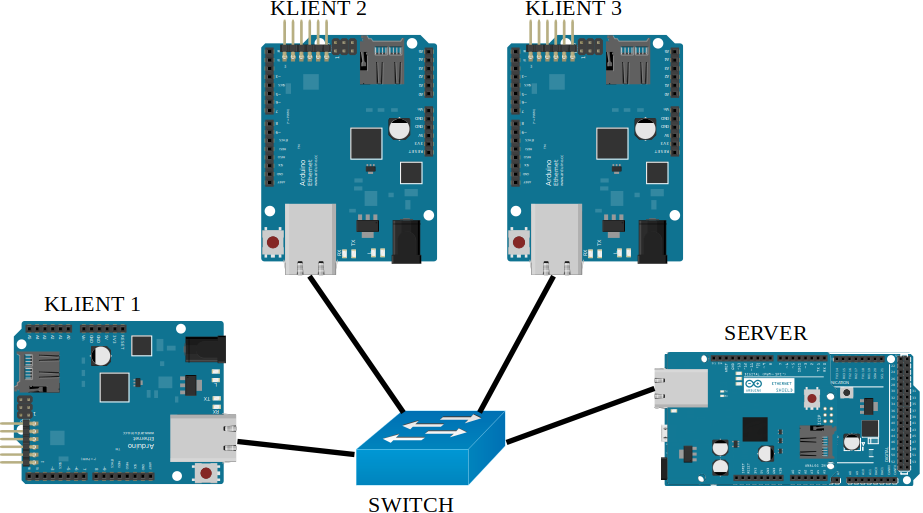
\includegraphics[width=7.5cm]{img/schema_net.png}
 \caption{Schéma zapojení jednotlivých zařízení do sítě}
 \end{figure}
 \end{itemize}
\end{frame}

\begin{frame}
\frametitle{Realizace - server}
\begin{columns}[c]
 \column{.5\textwidth}
	\begin{figure}
		\centering
		
\includegraphics[width=\textwidth]{img/server_realizace.jpg}
	\end{figure}
%
 \column{.5\textwidth}
	\begin{table}
		\centering
		\includegraphics[width=\textwidth]{img/serverLED.png}
	\end{table}
\end{columns}
\end{frame}


\section{Diskuze}
\begin{frame}
\begin{center}
\vspace*{1cm}
{\bf Děkuji za pozonost!}\\
\vspace*{2cm}
{\bf\Large \FirstName{} \LastName{}}\\
{\tt \Email}
\vspace*{1cm}
\end{center}
\end{frame}
\end{document}